% main_preprint.tex: builds the public accepted version of main_iceic_residual.tex with IEEE's copyright
% notice for accepted papers in the top margin of page 1; the paper itself (main_iceic_residual.tex) is unchanged.
%   pdflatex main_preprint && bibtex main_preprint && pdflatex main_preprint && pdflatex main_preprint
\AddToHookNext{shipout/foreground}{%
  \put(0,-20){\makebox[\paperwidth]{\parbox[t]{0.86\paperwidth}{\centering\scriptsize
    Accepted at the 2027 International Conference on Electronics, Information, and Communication (ICEIC).
    \copyright~2027 IEEE. Personal use of this material is permitted. Permission from IEEE must be obtained
    for all other uses, in any current or future media, including reprinting/republishing this material for
    advertising or promotional purposes, creating new collective works, for resale or redistribution to
    servers or lists, or reuse of any copyrighted component of this work in other works.}}}}
\pdfinfo{/Title (When to Replan and How Much to Correct: Residual Reinforcement Learning for Disturbance Recovery in Vision-Language-Action Policies) /Author (Chang-Hoon Ji and Tae-Eui Kam)}
\documentclass[conference,a4paper]{IEEEtran}
\IEEEoverridecommandlockouts
% The preceding line is only needed to identify funding in the first footnote.
\usepackage{cite}
\renewcommand{\citedash}{]\nobreakdash--[}   % keep citation ranges such as [7]--[10] on one line
\usepackage{amsmath,amssymb,amsfonts}
\usepackage{graphicx}
\usepackage{textcomp}
\usepackage{xcolor}
\usepackage{booktabs}
\usepackage{url}
\usepackage{tikz}
\usetikzlibrary{arrows.meta,decorations.pathreplacing,calc,positioning}

% ICEIC 2027 format: 2-6 pages, two-column A4, font >= 10 pt. Fig. 1 is fig_overview_res.tex (TikZ);
% figures/res_forest.pdf and res_general.pdf come from scripts/fig_paper.py and figures/res_qual.pdf
% from scripts/qual_frames.py + scripts/fig_qual.py of the code release.

\begin{document}

\title{When to Replan and How Much to Correct:\\
Residual Reinforcement Learning for Disturbance\\
Recovery in Vision-Language-Action Policies
\thanks{This work was supported by grants from the Institute of Information \&
Communications Technology Planning \& Evaluation (IITP) funded by the Korea
government (MSIT) [Artificial Intelligence Research Hub Project,
No.~\mbox{RS-2024-00457882}; Artificial Intelligence Graduate School Program at
Korea University, No.~\mbox{RS-2019-II190079}; Information Technology Research
Center (ITRC) program, No.~\mbox{IITP-2026-RS-2024-00436857}] and by a grant
from the National Research Foundation of Korea (NRF) funded by the Korea
government (MSIT) (No.~\mbox{RS-2023-00212498}).}
}

\author{\IEEEauthorblockN{Chang-Hoon Ji}
\IEEEauthorblockA{\textit{Department of Artificial Intelligence} \\
\textit{Korea University}\\
Seoul, Republic of Korea \\
ckdgns0611@korea.ac.kr}
\and
\IEEEauthorblockN{Tae-Eui Kam}
\IEEEauthorblockA{\textit{Department of Artificial Intelligence} \\
\textit{Korea University}\\
Seoul, Republic of Korea \\
kamte@korea.ac.kr}
}

\maketitle

% No footnotes in the abstract; pi_0.5 is typeset as bold math (the abstract is bold) by the authors' choice
% (the IEEE template asks for none; the EDAS abstract field keeps plain 'pi0.5').
\begin{abstract}
Vision-language-action policies that predict action chunks execute them open loop, so after an object is suddenly displaced, the robot follows a plan made for the old scene. On LIBERO\nobreakdash-10, teleporting the target object by 4 to 6\,cm, mostly as the gripper approaches, cuts the success of {\boldmath$\pi_{0.5}$} from 95 to 65 percent. Fixed inference-time settings for replan frequency, integration steps and chunk selection recover little. More computation at the next scheduled query recovers nothing measurable; replanning when a learned camera-frame detector fires adds no policy queries per episode and recovers zero to three points. When to replan matters less than how much to correct: a fixed-rule shift toward the estimated displacement gains about six points. Our event-gated residual is cloned from a scripted shift given the true displacement, refined with reinforcement learning as lightweight post-training and distilled into a vision-only student. In a pre-registered test on 500 fresh initial states, it raises success from 65.4 to 73.7 percent, a paired gain of 8.4 points, 95 percent interval 5.6 to 11.2. It beats the fixed-rule shift by 2.9 and does not measurably change undisturbed success.
\end{abstract}

\begin{IEEEkeywords}
action chunking, disturbance detection, event-triggered replanning,
post-training, residual reinforcement learning, vision-language-action models
\end{IEEEkeywords}

% =====================================================================
\section{Introduction}
% =====================================================================

Vision-language-action (VLA) models have become a common approach to
language-conditioned manipulation~\cite{kim2024openvla,black2024pi0,pi05}.
Most now predict \emph{action chunks}~\cite{zhao2023act,chi2025diffusion}:
one query of the model yields $H$ actions, of which the robot
executes only the first $h\le H$ and discards the rest before the model is queried again. Chunking smooths motion and amortizes the backbone's cost but makes the
controller open loop between queries. If a person moves an object
mid-chunk, the robot executes actions planned for the old scene
until the chunk is spent, and the next query sees a configuration the training data
rarely contains.

% =====================================================================
% fig_overview_res.tex -- Fig. 1 of the residual-recovery paper (TikZ).
% Requires in the preamble:
%   \usepackage{tikz}
%   \usetikzlibrary{arrows.meta,decorations.pathreplacing,calc,positioning}
% =====================================================================
\begin{figure*}[t]
\centering
\definecolor{cexec}{RGB}{0,114,178}
\definecolor{cevent}{RGB}{213,94,0}
\definecolor{ctrig}{RGB}{230,159,0}
\definecolor{cres}{RGB}{0,158,115}
\definecolor{cvla}{RGB}{86,180,233}
\definecolor{creg}{RGB}{204,121,167}
\resizebox{0.97\textwidth}{!}{%
\begin{tikzpicture}[
  >={Stealth[length=4pt,width=3pt]},
  font=\footnotesize,
  cell/.style={draw=black!55, line width=0.3pt, minimum width=0.30cm,
               minimum height=0.30cm, inner sep=0pt, outer sep=0pt},
  exe/.style={cell, fill=cexec!55},
  old/.style={cell, fill=cexec!18,
    path picture={\draw[black!45, line width=0.3pt]
      (path picture bounding box.south west) --
      (path picture bounding box.north east);}},
  cor/.style={cell, fill=cres!45},
  qry/.style={draw=ctrig!70!black, fill=ctrig!60, line width=0.3pt,
              rounded corners=1pt, minimum height=0.26cm, minimum width=0.16cm,
              inner sep=0pt},
  box/.style={draw=black!60, line width=0.4pt, rounded corners=2pt,
              align=center, inner sep=2.5pt, font=\footnotesize},
  lbl/.style={font=\footnotesize},
  flow/.style={->, line width=0.5pt}
]

% ------------------------------------------------------------------
% Panel (a): three reactions to a displacement inside a chunk
% ------------------------------------------------------------------
\def\w{0.30}      % cm per control step
\def\xo{2.55}     % x of the first action of chunk i
\def\td{4}        % displacement happens after action 4 of chunk i

% row (i): scheduled replanning (baseline)
\def\yA{0}
\node[lbl, anchor=east, align=right] at (\xo-0.1,\yA)
  {(i) scheduled replan\\[-1pt] (baseline)};
\foreach \t in {0,...,3} \node[exe] at ({\xo+(\t+0.5)*\w},\yA) {};
\foreach \t in {4,...,9} \node[old] at ({\xo+(\t+0.5)*\w},\yA) {};
\node[qry] at ({\xo+10*\w},\yA) {};
\foreach \t in {10,...,16} \node[exe] at ({\xo+(\t+0.5)*\w},\yA) {};
\node[lbl, anchor=west] at ({\xo+17*\w+0.1},\yA) {stale chunk runs out};

% row (ii): event-triggered replanning
\def\yB{-0.62}
\node[lbl, anchor=east, align=right] at (\xo-0.1,\yB)
  {(ii) replan at the\\[-1pt] event (detector)};
\foreach \t in {0,...,3} \node[exe] at ({\xo+(\t+0.5)*\w},\yB) {};
\node[old] at ({\xo+4.5*\w},\yB) {};
\node[qry] at ({\xo+5*\w},\yB) {};
\foreach \t in {5,...,16} \node[exe] at ({\xo+(\t+0.5)*\w},\yB) {};
\node[qry] at ({\xo+15*\w},\yB) {};
\node[lbl, anchor=west] at ({\xo+17*\w+0.1},\yB) {$+2.8$ pts ($+0.2$ fresh)};

% row (iii): event-triggered replanning + residual correction
\def\yC{-1.24}
\node[lbl, anchor=east, align=right] at (\xo-0.1,\yC)
  {(iii) + residual\\[-1pt] correction};
\foreach \t in {0,...,3} \node[exe] at ({\xo+(\t+0.5)*\w},\yC) {};
\node[old] at ({\xo+4.5*\w},\yC) {};
\node[qry] at ({\xo+5*\w},\yC) {};
\foreach \t in {5,...,16} \node[cor] at ({\xo+(\t+0.5)*\w},\yC) {};
\node[qry] at ({\xo+15*\w},\yC) {};
\node[lbl, anchor=west] at ({\xo+17*\w+0.1},\yC) {$+9.6$ pts ($+8.4$ fresh)};

% displacement marker
\draw[cevent, line width=0.6pt] ({\xo+\td*\w},\yA+0.25) -- ({\xo+\td*\w},\yC-0.25);
\node[lbl, cevent, above] at ({\xo+\td*\w},\yA+0.24) {object displaced 4--6\,cm};
\draw[decorate, decoration={brace, amplitude=2.5pt, mirror}, line width=0.4pt, cres!80!black]
  ({\xo+5*\w},\yC-0.22) -- node[lbl, below=1.5pt, cres!80!black]
  {$a_t\leftarrow a_t+\Delta$ for the next 6 queries} ({\xo+17*\w},\yC-0.22);

% time axis
\def\yT{-2.05}
\draw[->, line width=0.4pt] (\xo,\yT) -- ({\xo+17*\w+0.3},\yT);
\foreach \t in {0,5,10,15} {
  \draw[line width=0.3pt] ({\xo+\t*\w},\yT) -- ({\xo+\t*\w},\yT-0.06);
  \node[lbl, below] at ({\xo+\t*\w},\yT-0.03) {\t};}
\node[lbl, anchor=west] at ({\xo+17*\w+0.35},\yT) {control step};

% legend
\node[exe] at (0.35,-2.62) {};  \node[lbl, anchor=west] at (0.55,-2.62) {executed action};
\node[old] at (2.75,-2.62) {};  \node[lbl, anchor=west] at (2.95,-2.62) {planned before the event};
\node[cor] at (6.45,-2.62) {};  \node[lbl, anchor=west] at (6.65,-2.62) {corrected};
\node[qry, minimum width=0.16cm] at (8.15,-2.62) {}; \node[lbl, anchor=west] at (8.35,-2.62) {policy query};

\node[font=\footnotesize] at (4.6,-3.1)
  {(a) Reactions to a displacement inside a chunk ($H{=}h{=}10$)};

% ------------------------------------------------------------------
% Panel (b): vision-only pipeline and its training
% ------------------------------------------------------------------
\def\xb{11.0}

\node[box, fill=ctrig!15, draw=ctrig!70!black, minimum width=1.9cm] (det) at (\xb+1.7,0.05)
  {disturbance detector\\ CNN, every step};
\node[box, fill=cvla!15, draw=cvla!70!black, minimum width=1.9cm] (vla) at (\xb+5.9,0.05)
  {$\pi_{0.5}$ policy\\ query $\rightarrow$ chunk $\mathbf{A}$};
\node[box, fill=creg!15, draw=creg!70!black, minimum width=1.9cm] (reg) at (\xb+1.7,-1.25)
  {displacement regressor\\ CNN on the event frames};
\node[box, fill=cres!15, draw=cres!70!black, minimum width=1.9cm] (res) at (\xb+5.9,-1.25)
  {residual MLP\\ $\Delta=\mathbf{s}\odot\tanh u(\tilde x)$};
\node[circle, draw=black!60, line width=0.4pt, inner sep=0pt, minimum size=0.26cm, font=\scriptsize] (sum)
  at (\xb+7.75,-0.6) {$+$};
\node[box, fill=black!5, minimum height=1.9cm, minimum width=0.5cm, inner sep=1pt] (rob) at (\xb+8.45,-0.6)
  {\rotatebox{90}{robot}};

\node[lbl, align=center] (obsin) at (\xb+1.7,0.92) {frames $o_{t-1},o_t$ (2 cameras), $a_{t-1}$, end-effector motion};
\node[lbl] (vlain) at (\xb+5.9,0.92) {$o_t,\ell$};
\draw[flow] (obsin.south) -- (det.north);
\draw[flow] (vlain.south) -- (vla.north);
\draw[flow] (det) -- node[lbl, above, inner sep=1pt] {replan} (vla);
\draw[flow] (det) -- node[lbl, right] {event frames} (reg);
\draw[flow] (reg) -- node[lbl, above] {$\hat d$} (res);
\draw[flow] (vla.east) -| (sum.north);
\draw[flow] (res.east) -| (sum.south);
\draw[flow] (sum) -- (rob);
\node[lbl, anchor=north, align=center] at (\xb+4.35,-1.7)
  {$\tilde x$: proprio, chunk statistics, $\hat d$, queries since the event, task};

% training strip
\node[box, fill=white, inner sep=1.5pt, align=left] (train)
  at (\xb+4.35,-2.5)
  {training in simulation: scripted shift $0.5\,d$ $\rightarrow$ BC $\rightarrow$ PPO teacher (privileged $d$)\\[-1pt]
   $\rightarrow$ DAgger $\rightarrow$ vision-only student; detector, regressor: supervised};

\node[font=\footnotesize] at (\xb+4.35,-3.1) {(b) Vision-only system: when to replan, how much to correct};

\end{tikzpicture}%
}
\caption{Overview. (a) A chunked policy queried every $h$ actions
cannot react to a displacement until the current chunk is spent (i).
A learned detector interrupts the chunk and replans at the event (ii), and a residual policy adds a small correction $\Delta$ to every action of the
following queries (iii). (b) All three learned modules use only camera
frames, actions, proprioception and the task; the
$\pi_{0.5}$ weights are not updated. Gains: held-out initial states as in Fig.~\ref{fig:forest} (fresh in parentheses).}
\label{fig:overview}
\end{figure*}


How large is this cost, and what recovers it? We study the question with the
official $\pi_{0.5}$ checkpoint for LIBERO~\cite{pi05,liu2023libero} under
a controlled disturbance: a target object is teleported 4\nobreakdash--6\,cm horizontally, mostly when the open gripper first comes within 12\,cm of it.
Success on LIBERO-10 drops from 95.4\% to 64.7\%. Tracking the object
(Section~\ref{sec:diag}) shows that the policy often first closes the gripper nearer the \emph{old} position and that failures time out regrasping.

Recent work offers several responses, rarely compared under one disturbance. Adaptive-inference methods decide
when to replan, how much to compute per query or which sampled chunk to keep~\cite{liang2026aac,pan2026corrector,chun2025dasip,liu2025bid}; runtime
monitors detect execution failures~\cite{agia2024sentinel,xu2025faildetect,gu2025safe};
and residual reinforcement learning (RL) learns corrections on top of a fixed policy~\cite{yuan2025decorator,xiao2025pld}.
A concurrent benchmark of mid-execution changes such as target relocation finds that varying the replan frequency does not close the gap for four of its 14 policies, including $\pi_{0.5}$, but tests no event-triggered replanning or action correction~\cite{zhang2026liberomax}. We test both under one protocol, along with fixed settings of the inference levers. Replanning at the event helps little, and the new chunk seems to retarget the moved object only partly. Correcting the actions recovers more: about six of the 31 lost points with a fixed-rule shift and eight to ten with an event-gated residual policy learned as post-training around the VLA (Fig.~\ref{fig:overview}; Table~\ref{tab:rec}).

Our contributions are:
\begin{itemize}
  \item an evaluation protocol for mid-execution target displacement on LIBERO-10: every method faces the same seeded displacement and is compared with a seven-seed mean
        of $\pi_{0.5}$ alone
        (complementing setup~\cite{fei2025liberoplus} and action perturbations~\cite{guo2026robustvla,gao2026ogpo}; cf.\ \mbox{LIBERO-MAX}~\cite{zhang2026liberomax});
  \item evidence that when to replan matters less than how much to correct: inference levers recover little,
        more computation at the next scheduled query recovers nothing measurable and replanning at the detected event
        at most a few points, whereas a fixed-rule shift gains about six;
  \item an event-gated residual recovery policy that beats a fixed-rule shift by 2.9 points in a pre-registered
        test on fresh initial states, still gains with displacements twice as large and does not measurably change
        undisturbed success: as post-training around the VLA, we train a privileged teacher
        by behavior cloning (BC) of a scripted shift and then by proximal policy optimization (PPO), and distill it into a vision-only student gated by a learned per-step detector that detects 87--90\% of displacements on held-out
        initial states within three control steps.\footnote{Code, trained modules and per-episode results:\newline \url{https://github.com/BitAdventurer/VLA-Disturbance-Recovery}}
\end{itemize}

% =====================================================================
\section{Related Work}\label{sec:related}
% =====================================================================

\noindent\textbf{Adaptive chunk execution.}
AAC sets the executed prefix of a chunk from the entropy of sampled
chunks~\cite{liang2026aac}, and DVAC replans before the high-variance
actions of a chunk~\cite{feng2026dvac}. Bidirectional decoding selects among chunks
resampled at every step~\cite{liu2025bid}, RTC inpaints the next chunk
while the current one executes~\cite{black2025rtc}, and DA-SIP chooses the number of integration
steps per query with a difficulty classifier~\cite{chun2025dasip}. All five balance reactivity, consistency and compute but detect no events. VLA-Corrector~\cite{pan2026corrector} does: it truncates the chunk when visual latents drift from a learned prediction and replans with gradient guidance, but tests displacement only on hardware and adds no correction policy.

\noindent\textbf{Runtime monitoring.}
To flag failures or halt the policy, Sentinel~\cite{agia2024sentinel} checks action consistency and task progress, FAIL-Detect~\cite{xu2025faildetect} runs sequential out-of-distribution tests and SAFE~\cite{gu2025safe} probes VLA features. Like VLA-Corrector, we use detection to \emph{act}, here on one external event.

\noindent\textbf{Correcting a fixed policy's actions.}
Residual RL~\cite{johannink2019residual} refines imitation-learned policies~\cite{yuan2025decorator,ankile2024resip} and a
frozen $\pi_0$, with the corrections then distilled into the VLA~\cite{xiao2025pld}; latent-noise RL steers $\pi_0$ without changing its weights~\cite{wagenmaker2025dsrl}. Other work post-trains the VLA itself with online
RL~\cite{chen2025conrft,guo2025irevla} or with offline RL to recover from errors~\cite{gao2026ogpo}. Online RL has been shown to help when an
object is moved mid-episode~\cite{liu2025rl4vla}. A training-free operator offsets and
compresses a chunk toward perceived motion~\cite{zhang2026pacepath}, the
closest analog of our fixed-rule shift; teleports are its stated weak case. \mbox{TRANSIC} gates a residual with a classifier learned from human interventions~\cite{jiang2024transic}; ours is zero except after a detected scene displacement,
distilled from a privileged teacher into a vision-only student as
in~\cite{ankile2024resip}, and compared with a fixed-rule shift.

% =====================================================================
\section{Setting and Diagnosis}\label{sec:diag}
% =====================================================================

\subsection{Chunked Execution and the Disturbance}
A flow-based VLA maps an observation $o_t$ and instruction $\ell$ to a
chunk $\mathbf{A}_t=(a_t,\dots,a_{t+H-1})$ by conditional generation~\cite{lipman2022flow,oh2026ptdiff}, integrating a learned velocity
field for $n$ Euler steps~\cite{black2024pi0}; the robot
executes $h\le H$ actions and queries again. We use the released $\pi_{0.5}$ LIBERO checkpoint of openpi~\cite{pi05} with
$H=10$ and, by default, $(n,h)=(2,10)$, which scores 95.4\% undisturbed in one draw of the sampling noise. \emph{Policy-query time} sums the round-trip latency of every query in an episode, measured offline per setting on one RTX 5090 (32.6\,ms at $n=2$, 44.1\,ms at $n=10$); it is an accounting figure, as simulation is synchronous. The openpi example setting $(10,5)$ reaches 91.9\% (three draws) at $2.8\times$ the policy-query time and loses as many points as $(2,10)$ under the displacement below (to 61.2\%, two draws).
Episodes follow the released script (520
control steps at 20\,Hz after 10 settling steps) on the 50 fixed initial
states of each of the ten tasks.

The \emph{object displacement} is applied once per episode: when the open gripper first comes within 12\,cm (end effector to object center)
of a movable object of interest (an object named in the task goal) that it
does not hold, that object is teleported horizontally by a distance drawn from
$[4,6]$\,cm in a uniformly random direction and its velocity is zeroed. If no approach has occurred by a random step in 50--170 (about 26\% of episodes, mostly in two tasks), a time fallback displaces the nearest free object of interest at that step. Direction and magnitude are seeded per task and initial state, so every method sees the same vectors. Every method except the fixed $(n,h)$ schedules of Section~\ref{sec:levers} reuses the noise seed of one base draw and matches its event step and displaced object in nearly every episode (a few pre-event trajectories differ). Event steps differ between base draws in 27\% of episodes and between a fixed schedule and a base draw in 46--56\%, mostly by one step. Success drops to 64.7\% (mean of seven noise draws); every
failure is a timeout.

\subsection{Why the Policy Fails}
Failures differ from successes not in where the gripper first closes but in whether a few regrasps succeed before time runs out (Table~\ref{tab:diag}). We tracked the displaced object in 100 disturbed episodes (initial states 0--9 of each task, one base draw). All successes eventually lift it, but 46\% of
failures never do. In about 62\% of \emph{both} groups the first gripper closure after the
event is nearer to the object's old position than to its new one, and even successful episodes at first move more toward the old position, while failures move decisively toward neither. More computation at the next scheduled query does not help (Section~\ref{sec:event}), although the new position is already visible there.
This suggests that a new query does not fully retarget the moved object and that the actions themselves need a shift; Section~\ref{sec:results} tests both.

\begin{table}[t]
\caption{Successful and Failed Episodes After the Displacement (100~Tracked Episodes)}
\label{tab:diag}
\centering
\footnotesize
\begin{tabular}{lcc}
\toprule
 & Success (65) & Failure (35) \\
\midrule
Displaced object eventually lifted & 100\% & 54\% \\
Gripper closures before lift or timeout & 2.3 & 7.7 \\
First closure nearer to the old position & 62\% & 63\% \\
Motion toward old / new position$^{\mathrm{a}}$ & 0.69 / 0.60 & 0.26 / 0.39 \\
\bottomrule
\multicolumn{3}{l}{\scriptsize $^{\mathrm{a}}$Mean cosine of end-effector motion with the direction to each} \\
\multicolumn{3}{l}{\scriptsize position over the 15 steps after the event.}
\end{tabular}
\end{table}

\subsection{Evaluation Protocol}\label{sec:protocol}
Flow-based policies sample the initial noise of the integration, and this
noise alone varies the success of $(2,10)$ on the disturbed episodes from 63.2\% to 67.8\% across seven seeds (``noise draws''). We compare every variant with the \emph{per-episode mean of the seven
noise draws} of the base policy on the same 500 (task, initial state) episodes with the same disturbance. We report the mean
paired difference with a task-stratified bootstrap 95\% interval in brackets (6,000
resamples). Variants run once carry their single draw's noise and resolve only
differences of several points. The detector, regressor and teachers are each trained once, and the students with three distillation seeds (the released one unless stated), all on training states 0--24 only. Results on all 500 episodes include these states. States 25--49 of the same ten tasks (250 episodes, base 62.2\%) are held out from training for the comparisons in Fig.~\ref{fig:forest}, but not from model selection: they also served to choose gates, shift scales and models. We therefore tested the released pipeline once, under a pre-registered protocol (in the code release), on 500 fresh episodes: states 50\nobreakdash--99 of each task's full initial-state file (the benchmark uses 0--49), unused by any earlier rollout of ours, with five base draws and two or three per method. No new task is tested. Intervals are per comparison, without multiplicity correction.

% =====================================================================
\section{Method}\label{sec:method}
% =====================================================================

\subsection{Detecting the Event and Replanning Immediately}
To replan at the event rather than at the next scheduled query, we run a detector beside the controller. At every control step, it receives the previous and current frames of both cameras (third-person and wrist) and their difference, in $64\times64$ grayscale, plus the action executed between them and the measured end-effector motion; a four-layer CNN and a small MLP fuse these into one
logit (0.1\,M parameters). All data come from training states: positives are the frame pairs straddling a displacement, hard negatives the pairs within 15 steps of it, plus the pairs of 130 undisturbed episodes. Training uses the 500 events of two disturbed runs, and the threshold is set for 0.05 false alarms per episode on 120 further undisturbed episodes.

When the logit crosses the threshold, the schedule interrupts the current
chunk and queries the policy immediately (Fig.~\ref{fig:overview}(a)). Policy-query time stays at $1.00\times$ the base schedule's (37.2 versus 37.4 queries per episode): each detection (1.07 per disturbed episode) adds at most one query (1.7\% more queries per step), but episodes end earlier on average.

\subsection{Residual Correction}
To shift the actions, we add a residual $\Delta\in\mathbb{R}^3$ to the translational part of every
action $a_j$ of the chunk returned by a query,
\begin{equation}
a_j^{\mathrm{xyz}} \leftarrow \mathrm{clip}(a_j^{\mathrm{xyz}}+\Delta,-1,1),\qquad
\Delta=\mathbf{s}\odot\tanh u(x),
\label{eq:residual}
\end{equation}
computed once per query from a feature vector $x$ by a two-layer MLP $u$ (256 units), with element-wise $\odot$ and $\mathbf{s}=(0.3,0.3,0.15)$ in LIBERO action units (0.3 units move the end effector by about 3.6\,mm per control step). The residual is \emph{gated}: it is zero except for a bounded window after
a detected displacement, so undisturbed behavior is touched only on false
alarms.

\noindent\textbf{Scripted shift (privileged).}
As a reference, once the simulator reports at a scheduled query that an unlifted object of interest has moved by $d$ (over 2\,cm) since the reset, we add a nominal $\alpha d$ of horizontal end-effector motion, split over the $kh$ actions of the $k$ chunks from this query on, without interrupting the chunk. With $k=2$, $\alpha=1$ and $0.5$ perform alike (71.2\% and 72.2\% on all 500, one draw) and $\alpha=1.5$ worse (64.8\%), presumably by adding to the base policy's own partial correction. A vision-only counterpart, the \emph{fixed-rule shift}, replans at each detection and adds $0.5\,\hat d$ likewise,
with $\hat d$ from the regressor below.

\noindent\textbf{Privileged teacher.}
We then learn the correction with residual RL~\cite{johannink2019residual} on privileged state. Choosing the residual at each gated query is a sequential decision problem, as in our earlier RL work~\cite{ji2026hrl,ji2024sparse,ji2026agentic}. The teacher's 53 inputs are proprioception, a summary of the base chunk, episode progress, gripper state, queries since the gate opened, the previous residual, a task one-hot and, for up to three objects of interest, their relative position, displacement and presence. At every scheduled query (no replan at the event), its gate
opens when an object has jumped more than 2.5\,cm since the previous query
while it rests within 1.5\,cm of its initial height and the open gripper is over 5\,cm away, and closes once the object is lifted 3\,cm. It
opens in 85\% of disturbed and in none of 250 undisturbed held-out episodes,
whereas a looser, cumulative 2\,cm gate opened in 54\% of the undisturbed ones; with that gate, a learned teacher (trained, like ours, only on disturbed episodes) cut undisturbed
success to 73.6\%. At gated query $i$ the actor samples $z_i\sim\mathcal{N}(u_\theta(x_i),\operatorname{diag}\boldsymbol{\sigma}^2)$ ($\boldsymbol{\sigma}$ initially 0.30) and applies $\Delta_i=\mathbf{s}\odot\tanh z_i$. We first clone the scripted residual $\Delta^{\mathrm{sh}}_i$ ($\alpha=0.5$, $k=2$, triggered by the teacher's gate) from 441 episodes by minimizing \eqref{eq:bc}, where $\oslash$ is element-wise division. We then run PPO with generalized advantage estimation~\cite{schulman2016gae} (settings in the code release) for 40 iterations of 120 episodes on training states. It maximizes \eqref{eq:ppo} with success $R\in\{0,1\}$ at the last of $T$ gated queries, $\gamma=0.99$ and a fixed rather than adaptive weight $c=0.01$~\cite{ji2026moreward,hwang2026arw}; one run takes about two GPU-hours.

\noindent\textbf{Vision-only student.}
The student may use neither object positions nor the privileged
gate (Fig.~\ref{fig:overview}(b)). Its gate is the learned detector: each detection, true or
false, costs one replan and opens (or restarts) a window of six queries. When the detector fires, a \emph{displacement regressor} (four ResNet blocks, 0.5\,M parameters) estimates the horizontal displacement $\hat d$ from the $128\times128$ RGB frame pairs of both cameras, the executed action and the end-effector motion at that step. Trained on 1,499 events of 2\nobreakdash--10\,cm from training states, it has a median error of 1.6\,cm and $9^\circ$ in direction on 1,499 events from held-out initial states (median displacement 6.0\,cm). The student MLP $u_\phi$ sees the teacher's inputs with the object state replaced by $\hat d$, its norm and an active flag (36 inputs $\tilde x$, fusing $\hat d$ with the base chunk~\cite{kang2026fusion}). It is trained with dataset aggregation (DAgger)~\cite{ross2011dagger} to match the teacher's greedy residual $\Delta^\star_i=\mathbf{s}\odot\tanh u_\theta(x_i)$, zero outside the teacher's gate, in three rounds of two rollouts per training state (10\% undisturbed) under the student's gate. The teacher's residual replaces the student's at each gated query with probability $\beta=1,0.5,0$ per round. Round $r$ minimizes \eqref{eq:distill} over the student-gated queries $\mathcal{D}_{\le r}$ of rounds up to $r$ (8,148 labels after three). The three objectives are
\begin{align}
\mathcal{L}_{\mathrm{BC}}(\theta)&=\textstyle\sum_i\big\|u_\theta(x_i)-\operatorname{artanh}(\Delta^{\mathrm{sh}}_i\oslash\mathbf{s})\big\|^2,\label{eq:bc}\\
J(\theta)&=\mathbb{E}\big[\gamma^{T-1}R-c\textstyle\sum_{i=0}^{T-1}\gamma^{i}\big\|\Delta_i\oslash\mathbf{s}\big\|^2\big],\label{eq:ppo}\\
\mathcal{L}_{\mathrm{DAgger}}(\phi)&=\textstyle\sum_{i\in\mathcal{D}_{\le r}}\big\|\mathbf{s}\odot\tanh u_\phi(\tilde x_i)-\Delta^\star_i\big\|^2.\label{eq:distill}
\end{align}

% =====================================================================
\section{Results}\label{sec:results}
% =====================================================================

\begin{figure}[t]
\centering
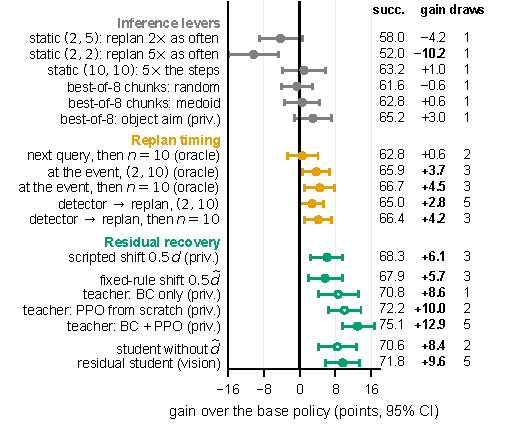
\includegraphics[width=\columnwidth]{figures/res_forest.pdf}
\caption{Gain over the base policy $(2,10)$, the mean of seven noise draws (62.2\%), on the 250 held-out disturbed episodes; task-stratified paired
bootstrap 95\% intervals. $(n,h)$: integration steps and executed actions per query; ``oracle'': event time from the simulator; ``priv.'': uses simulator state; ``static'': fixed
schedule; hollow: ablations. Right: success, gain (bold: interval excludes zero), noise draws.}
\label{fig:forest}
\end{figure}

\subsection{Inference Levers Recover Little}\label{sec:levers}
We test fixed settings of the levers that adaptive-inference methods tune, not those methods themselves (Fig.~\ref{fig:forest}, top, held out). Replanning twice as often, $(2,5)$, trends down ($-4.2$); five times as often, $(2,2)$, loses ten points. Five times as many integration steps, $(10,10)$, change nothing measurable ($+1.0$). Selecting one of $K=8$ sampled chunks for the seven queries after the (oracle-timed) event also recovers little: random $-0.6$, medoid $+0.6$, a privileged rule aiming at the displaced object $+3.0$. On all 500, $(2,2)$ scores 87.9\% undisturbed, and every schedule tested falls 29\nobreakdash--33 points below its own undisturbed success.

\subsection{When to Replan: At Most a Few Points}\label{sec:event}
The base policy already replans at the next scheduled query. On held-out episodes, spending $n=10$ steps on that query and up to two more (oracle event timing) gains nothing measurable ($+0.6$ [$-2.6$,~$+4.1$]). With the same oracle, replanning \emph{at} the event gains $+3.7$ at $(2,10)$; with $n=10$ on the three queries from the event, it gains $+4.5$, which is $+3.9$ [$+0.4$,~$+7.3$] above the next-query variant. In closed loop, the learned detector flags 87--90\% of the displacements on held-out initial states within three control steps (98--100\% on training states), with 0.10--0.15 false alarms per disturbed episode. Without the oracle, it keeps most of the oracle's gain ($+2.8$ and $+4.2$; all 500: Table~\ref{tab:rec}) at $1.00\times$ and $1.02\times$ the policy-query time. On fresh initial states its replan gains only $+0.2$ [$-2.4$,~$+2.8$], so the small gain above is not confirmed.

\subsection{How Much to Correct: Larger Gains}\label{sec:correct}
Shifting the actions adds to replanning. With privileged $d$, the detector's replan plus the scripted shift reaches 71.3\% held out (three draws), $+6.4$ [$+2.9$,~$+10.1$] above the replan alone. The privileged scripted shift and the fixed-rule shift by $0.5\,\hat d$, which adds a replan at each detection, gain about the same (held out: $+6.1$, $+5.7$; Fig.~\ref{fig:forest}). Learning the correction helps further. Held out, the privileged teacher, whose correction is longer and more gradual than the scripted shift's, gains $+12.9$ [$+9.5$,~$+16.6$] and is $+4.3$ [$+0.5$,~$+8.4$] above its behavior-cloned start. PPO from scratch is 2.9 points [$-0.4$,~$+6.3$] below the teacher. We did not distill a student from the behavior-cloned start, so PPO's share of the student's gain is not measured.

Without any privileged input, the distilled student comes within a few points of its teacher and beats the fixed-rule shift. In the pre-registered test on fresh initial states (Table~\ref{tab:rec}), it gains $+8.4$ [$+5.6$,~$+11.2$] over the base policy and $+2.9$ [$+0.7$,~$+5.1$] over the fixed-rule shift; undisturbed success changes by $-0.2$ [$-1.0$,~$+0.4$] (one draw). Held out, it gains $+9.6$ [$+5.8$,~$+13.4$] and is $-4.4$ [$-7.3$,~$-1.6$] against a teacher that also replans at each detection (76.1\%). The student is $+3.9$ [$+0.9$,~$+6.9$] against the fixed-rule shift and $+3.9$ [$+1.2$,~$+6.8$] against the best of seven rules chosen on training states ($\alpha=0.5$, $k=4$; all 500: $+4.7$, $+4.8$). On all 500 undisturbed episodes the student (active in 5\% through false alarms) scores 95.4\%, as does the base draw with the same noise; against three base draws it is $+0.3$ [$-1.0$,~$+1.7$], so the 95\% interval excludes drops above about one point. Against the 32.6\,ms GPU policy query, the detector takes 0.4\,ms per control step, the regressor 2.2\,ms per detection and the student MLP 0.02\,ms per active query (two CPU threads; full loop not timed).

\begin{table}[t]
\caption{Summary of Results per Set of Initial States: Success of $\pi_{0.5}$ Alone (\%) and Paired Gains (Points)}
\label{tab:rec}
\centering
\scriptsize
\setlength{\tabcolsep}{2.2pt}
\begin{tabular}{llccccc}
\toprule
 & & Fresh$^{\mathrm{a}}$ & Held out & All & 8--12\,cm & Undist. \\
Method & In. & 50--99 & 25--49 & 0--49 & 0--49 & 0--49 \\
\midrule
$\pi_{0.5}$ alone, $(2,10)$ & -- & 65.4 & 62.2 & 64.7 & 37.0 & 95.4 \\
Detector $\rightarrow$ replan & V & $+0.2$ & $\mathbf{+2.8}$ & $\mathbf{+2.5}$ & -- & $-0.2$ \\
Detector $\rightarrow$ replan, then $n{=}10$ & V & -- & $\mathbf{+4.2}$ & $\mathbf{+3.3}$ & -- & -- \\
Scripted shift $0.5\,d$ & P & -- & $\mathbf{+6.1}$ & $\mathbf{+6.3}$ & -- & $\mathbf{-4.6}$ \\
Fixed-rule shift $0.5\,\hat d$ & V & $\mathbf{+5.4}$ & $\mathbf{+5.7}$ & $\mathbf{+6.5}$ & $\mathbf{+3.8}$ & $0.0$ \\
Residual teacher (BC + PPO) & P & -- & $\mathbf{+12.9}$ & $\mathbf{+12.7}$ & $\mathbf{+12.1}$ & $-0.2$ \\
Student without $\hat d$ & V & -- & $\mathbf{+8.4}$ & $\mathbf{+9.8}$ & $\mathbf{+4.4}$ & $0.0$ \\
\textbf{Residual student} & V & $\mathbf{+8.4}$ & $\mathbf{+9.6}$ & $\mathbf{+11.2}$ & $\mathbf{+8.3}$ & $0.0$ \\
\bottomrule
\multicolumn{7}{l}{\scriptsize Held out: 250 episodes, other columns 500. Bold: 95\% interval excludes zero.} \\
\multicolumn{7}{l}{\scriptsize In.: V vision + proprioception, P privileged state. $^{\mathrm{a}}$Pre-registered test.} \\
\multicolumn{7}{l}{\scriptsize Draws: base 3--7, methods 2--5; Undist.: one each, base seed (base, 3 draws: 95.1).}
\end{tabular}
\end{table}

\subsection{Other Disturbances and Side Effects}
Trained only on 4--6\,cm displacements, mostly during the approach, the student still gains with displacements twice as large and is neutral on the other disturbances (Fig.~\ref{fig:general}; all 500, modules unchanged). With 8--12\,cm displacements (base 37.0\%), it gains $+8.3$ [$+5.0$,~$+11.5$], which is $+4.5$ [$+1.5$,~$+7.5$] more than the fixed-rule shift and $+4.2$ more than the best of seven rules. Beyond the regressor's 10\,cm training range the student still gains $+8.0$ [$+3.7$,~$+12.4$] ($+7.7$ [$+1.9$,~$+13.6$] on held-out initial states). For a late move of the nearest free object (steps 110--210), the detector fires in half of the episodes and the student's gain is within noise ($+1.4$), whereas the privileged teacher is slightly harmful ($-2.4$ [$-4.2$,~$-0.5$]; two draws each). For a five-step arm push and for sliding (6\nobreakdash--10\,cm planned, cut short when the gripper closes, so slides differ by method), the teleport-trained detector rarely fires (6\nobreakdash--12\%), and success changes by at most 1.1 points. Undisturbed success is 95.2--95.6\% in every detector-gated variant on states 0--49: the detector gate bounds how often a residual can act, whereas the scripted shift's cumulative gate costs 4.6 points (90.8\%).

\begin{figure}[t]
\centering
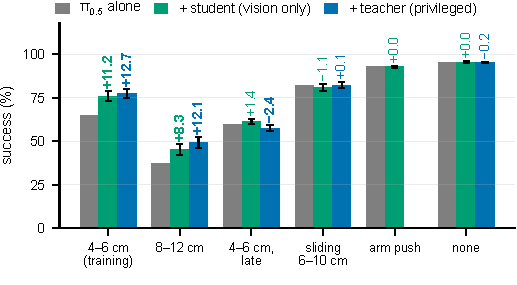
\includegraphics[width=\columnwidth]{figures/res_general.pdf}
\caption{Success under the training disturbance (left), other disturbances and ``none'' (500 episodes each; draws, baseline/methods: 7/5 at 4--6\,cm, 3/2 at \mbox{8--12\,cm}, 2/2 late, 2/1 sliding, 1/1 otherwise). Numbers: paired gains; whiskers: 95\% intervals; bold: interval excludes zero.}
\label{fig:general}
\end{figure}

\begin{figure}[t]
\centering
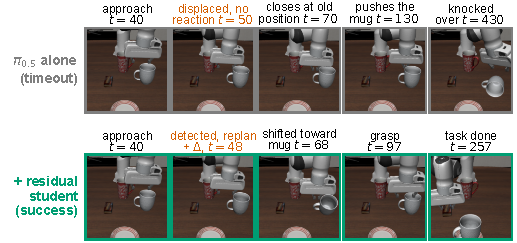
\includegraphics[width=\columnwidth]{figures/res_qual.pdf}
\caption{One held-out episode of the mug-and-pudding task, with the same sampling noise in both rows; $t$: control step; the mug moves at $t=47$. Top: $\pi_{0.5}$ alone (timeout). Bottom: with the detector and residual student (success).}
\label{fig:qual}
\end{figure}

\subsection{Ablation: Displacement Estimate}
A student distilled without $\hat d$ is only slightly worse than the full one on all 500 ($-1.4$ [$-3.5$,~$+0.9$], two draws; $-1.4$ to $-2.8$ over three distillation seeds): at 4--6\,cm the detector tells it \emph{when}, while the base chunk, proprioception and the task input may tell it \emph{how}. At 8--12\,cm, removing $\hat d$ hurts in two of three seeds ($-3.9$ [$-6.5$,~$-1.3$], two draws; other seeds $-6.0$, $+0.8$). But $\hat d$ does not make the correction proportional: held out, from 4--6 to 8--12\,cm the student's shift along the displacement grows only from 2.3 to 3.2\,cm (the teacher's from 3.3 to 9.2\,cm), as $\hat d$ saturates near 6\,cm.

\subsection{Where the Residual Helps and Where It Fails}
Gains concentrate where the approach triggers the event. Held out, the student gains $+12.3$ [$+7.6$,~$+17.1$] on the 179 approach-triggered episodes but $+2.7$ [$-2.6$,~$+7.9$] on the 71 triggered by the time fallback (fresh initial states: $+11.3$ and $-0.1$). In Fig.~\ref{fig:qual}, $\hat d$ is poor (1\,cm, wrong direction), yet the correction points toward the mug, so its direction may come from the base chunk or a task-level push. The residual was active in 85\% of the student's remaining held-out failures, so few are due to missed detections; a likely bottleneck is the correction itself, whose DAgger labels are zero where the teacher's gate stayed closed.


% =====================================================================
\section{Conclusion}
% =====================================================================

After the target object is displaced, $\pi_{0.5}$ loses 31 points, and its failures time out regrasping. When to replan matters less than how much to correct: replanning at the detected event recovers zero to three points, a
fixed-rule shift about six and, on fresh initial states, the event-gated residual student about eight. Gating keeps our post-training conservative: undisturbed success does not measurably change, whereas a loosely gated teacher cut it to 73.6\%. We test only one policy, benchmark and task set, mostly with single training runs. Needing no object state and little CPU time, the modules could run beside a robot's VLA, like \mbox{TRANSIC}'s residual beside a simulation-trained policy~\cite{jiang2024transic}. Open sim-to-real gaps are rendered training frames, teleported rather than physical displacements, and synchronous execution; next, we will probe them on hardware, make the correction track the displacement and try an end-to-end, possibly multi-agent gate~\cite{shin2024mars}.

\bibliographystyle{IEEEtran}
\bibliography{refs_res}

\end{document}

